
\documentclass[border=10pt]{standalone}
\usepackage{pgfplots}
\pgfplotsset{compat=1.17}
\usetikzlibrary{patterns}
\begin{document}
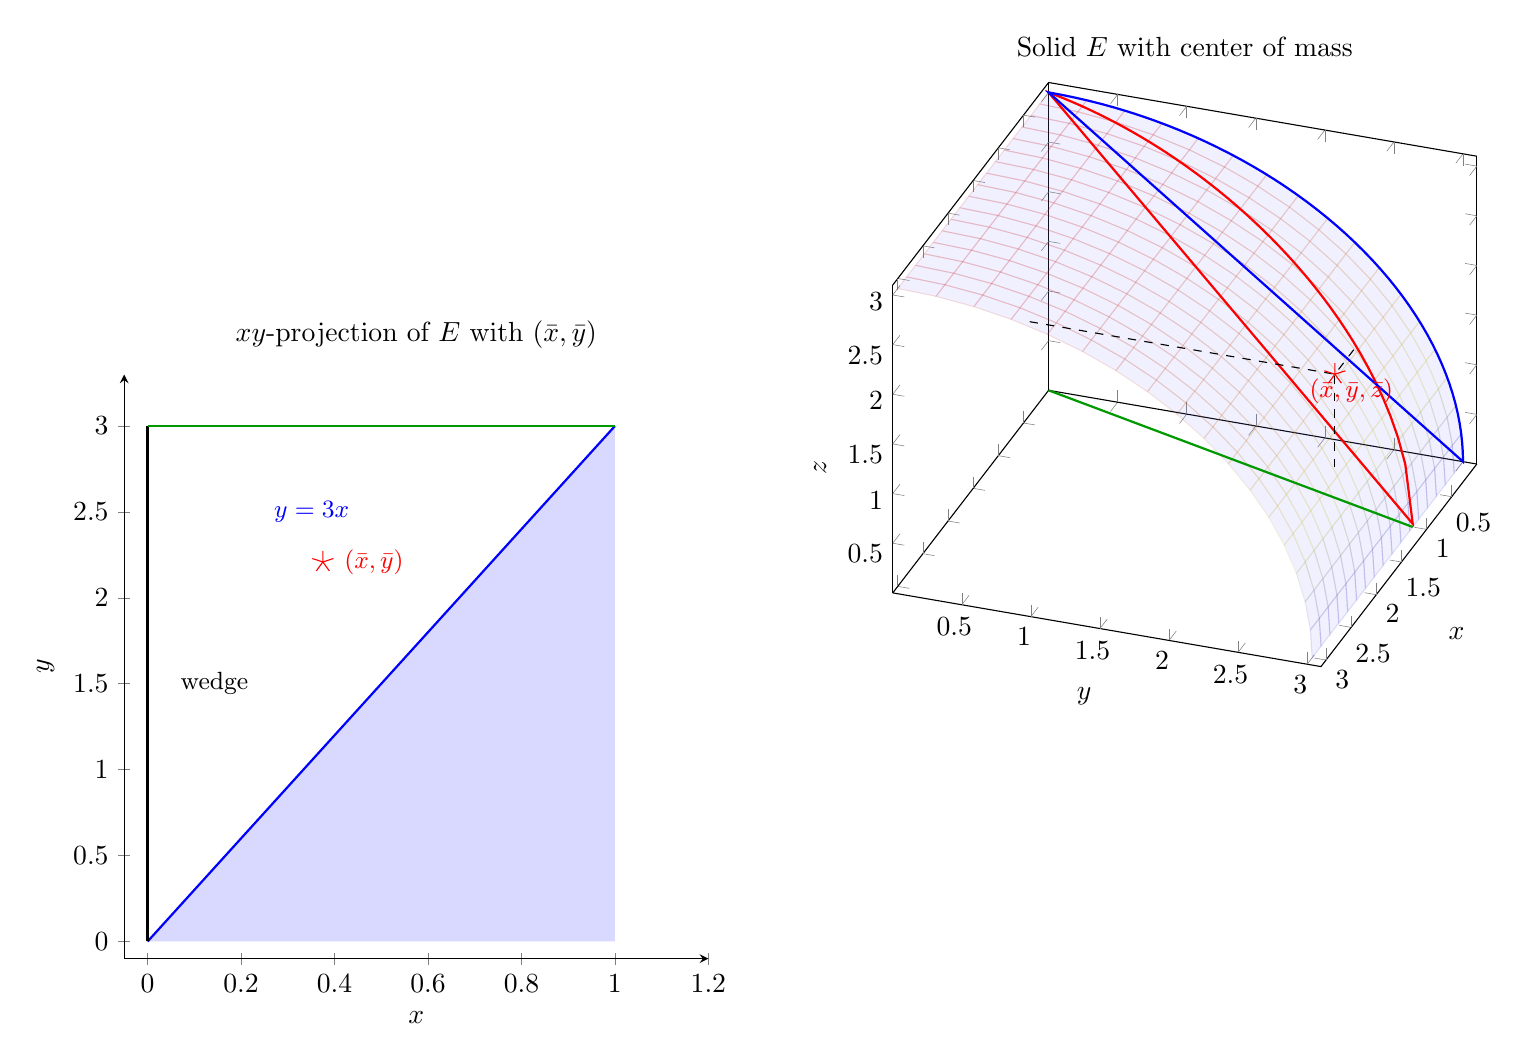
\begin{tikzpicture}

% ----- 2D: xy-projection with center of mass marked -----
\begin{axis}[
    name=plot2d,
    xlabel={$x$}, ylabel={$y$},
    xmin=-0.05, xmax=1.2, ymin=-0.1, ymax=3.3,
    width=9cm, height=9cm,
    axis lines=left,
    title={$xy$-projection of $E$ with $(\bar x, \bar y)$},
    legend pos=south east,
]
% Region projection: y from 0 to 3, x from 0 to y/3
\addplot[domain=0:3, samples=2, fill=blue!15, draw=none] ({x/3}, {x}) \closedcycle;

% Boundary lines
\addplot[domain=0:3, samples=10, blue, thick] ({x/3}, {x});
\addplot[domain=0:3, samples=10, black, thick] ({0}, {x});
\addplot[domain=0:1, samples=10, green!60!black, thick] ({x}, {3});

% Center of mass point
\addplot[only marks, mark=star, mark size=4pt, color=red, mark options={fill=red}] 
    coordinates {(0.375, 2.209)};
\node[red, anchor=west] at (axis cs:0.4, 2.209) {\small $(\bar x, \bar y)$};

% Annotate
\node[anchor=west] at (axis cs:0.05, 1.5) {\small wedge};
\node[anchor=west, blue] at (axis cs:0.25, 2.5) {\small $y = 3x$};

\end{axis}

% ----- 3D view with center of mass -----
\begin{axis}[
    name=plot3d,
    at={(plot2d.right of east)}, xshift=2cm,
    view={110}{35},
    xlabel={$x$}, ylabel={$y$}, zlabel={$z$},
    xmin=0, xmax=3.1, ymin=0, ymax=3.1, zmin=0, zmax=3.1,
    width=9cm, height=9cm,
    title={Solid $E$ with center of mass},
    xtick={0.5,1,1.5,2,2.5,3},
    ytick={0.5,1,1.5,2,2.5,3},
    ztick={0.5,1,1.5,2,2.5,3},
]
% Quarter cylinder surface
\addplot3[
    domain=0:3, domain y=0:1.5708,
    samples=18, samples y=18,
    surf, z buffer=sort, opacity=0.12, color=blue!50
] ({x}, {3*cos(deg(y))}, {3*sin(deg(y))});

% Boundary curves
% Edge: y=3x on cylinder (red)
\addplot3[domain=0:1, samples=50, red, thick] ({x}, {3*x}, {3*sqrt(1-x^2)});
% x=0: blue
\addplot3[domain=0:1.5708, samples=50, blue, thick] ({0}, {3*cos(deg(x))}, {3*sin(deg(x))});
% z=0: green
\addplot3[domain=0:3, samples=10, green!60!black, thick] ({x/3}, {x}, {0});

% Center of mass
\addplot3[only marks, mark=star, mark size=4pt, color=red, mark options={fill=red}] 
    coordinates {(0.375, 2.209, 0.938)};
\node[red, anchor=west] at (axis cs:0.5, 2.0, 0.8) {\small $(\bar x, \bar y, \bar z)$};

% Dashed lines to coordinate planes
\addplot3[dashed, black, thin] coordinates {(0.375, 2.209, 0) (0.375, 2.209, 0.938)};
\addplot3[dashed, black, thin] coordinates {(0.375, 0, 0.938) (0.375, 2.209, 0.938)};
\addplot3[dashed, black, thin] coordinates {(0, 2.209, 0.938) (0.375, 2.209, 0.938)};

\end{axis}

\end{tikzpicture}
\end{document}
